\documentclass{article}


\usepackage[nottoc,numbib]{tocbibind}
\usepackage[utf8]{inputenc}
\usepackage{graphicx}
\usepackage{subcaption}
\usepackage{geometry}
\usepackage{amssymb}
\usepackage{caption}
\usepackage{float}
\usepackage{wrapfig}
\usepackage{romannum}
\usepackage{physics}
\usepackage{amsmath,amsfonts,amsthm,bm} % Math packages
\geometry{margin=1in}

\errorcontextlines 10000
\begin{document}
\pagenumbering{gobble}
\begin{titlepage}
    \begin{center}
        \vspace*{1cm}
        \Large

\includegraphics[width=.4\linewidth]{../logo.pdf}\\
        \Large
\vspace{1cm}
        Machine Learning Practicum\\
        \huge
        \textbf{Finding the Higgs' boson\\}
\Large  
        \vspace{1cm}
        \textbf{Andrej Kolar - Po{\v z}un\\}
        \vspace{0.8cm}

\vfill
\normalsize
\end{center}. 
\end{titlepage}
\newpage
\pagenumbering{arabic}
\section*{Intro}
ATLAS has found the Higgs' boson back in 2012. In this project we aim to replicate this by using their data from the LHC (Large Hadron Collider). 
Greatly simplifying, in the collider two streams of particles are sent towards each other and collisions (events) occur that are then recorded by the detectors. Our input data is merely the number of events in a given energy range.
A consequence of the Higgs' model is that one of the events is the decay of the Higgs into two muons, which happens at an energy of around $125 GeV$ (Higgs' mass). We woud like to find this event in our data.

The problem is that the number of the events at all energy scales (including the one near $125 GeV$ is huge (millions). How do we even begin to verify the theory and look for Higgs at such scale?
The answer is - with further predictions from theory. Using Monte Carlo (MC) techniques particle physicists are able to simulate how the Higgs' signal should look like (as a histogram over the energy - due to spectral broadening, we expect Higgs' related events not only at $125 GeV$, but also in it's vicinity.). We are also able to simulate how the background (known) processes should look like.

So what we are looking for is the Higgs' signal - a bump in the data at the expected energy and of expected shape. What makes that difficult is that the vast majority of the data (a factor of hundreds of events) are just background processes, which we will have to somehow subtract. 
\section*{Data}
From cernbox.cern.ch, we get the following data (.h5 files):
\begin{itemize}
\item Simulated background (num. of events / energy)
\item Simulated (Higgs') signal (num. of events / energy)
\item Actual measured data (num. of events / energy
\end{itemize}
The first step is to bin the input data and plot the histograms. The results can be seen on Figure below:
\begin{figure}[H]
\centering
\begin{subfigure}{.7\textwidth}
\includegraphics[width=\linewidth]{Pictures/all_hmumu_ratio.pdf}
\end{subfigure}
\caption*{On the top, experimental (black) and simulated data is shown. The lower plot shows that we have more actual events than the simulated background (bkg). Number of bins: 50.}
\end{figure}
Since we are interested only at the event happening near $125 GeV$, plotting and using the data from a full range of energies is unnecessary. Hence we will use only an energy range of $[110,160] GeV$ from now on, as this covers the interesting part, while still providing plenty of room for us to interpolate the background from (more on that later).
We must now decide on the number of bins, that we will use to construct the histograms. Some different choices are shown below:
\begin{figure}[H]
\centering
\begin{subfigure}{.32\textwidth}
\includegraphics[width=\linewidth]{Pictures/bins10.pdf}
\end{subfigure}
\begin{subfigure}{.32\textwidth}
\includegraphics[width=\linewidth]{Pictures/bins50.pdf}
\end{subfigure}
\begin{subfigure}{.32\textwidth}
\includegraphics[width=\linewidth]{Pictures/bins250.pdf}
\end{subfigure}
\caption*{Same plot as before for the interested region for 10 (left), 50 (center) and 250 (right) bins.}
\label{fig:diffBins}
\end{figure}
Increasing the number of bins, decreases the number of events/bin, which has an effect on error: For simulated data, the errors are provided (and thus, the total variance in the bin is just the sum of the individual variances of that bin's data), while the experimental data follows the Poisson distribution (limit of binomial distribution for huge $N$ and small $p$) so the variance is just equal to the number of events in that bin.
So the errors per bin decrease as we increase their number, but the error of the ratio (data/background) increases. We opt for the number of bins equal to $50$ as its errors are not so large yet and it seems to capture how the data looks like well enough.

\section*{Fitting the background}
From the previous pictures we could notice that the simulated background is not a very good fit to the data, even outside the Higgs' region. The difference is minimal, but still observable with naked eye and we need a more accurate model of the background to find the Higgs' signal (which, remember, is much smaller and could easily be smeared by wrong background). We will then be able to subtract the background from the experimental data.

Obviously the goal isn't just a perfect fit, which we could get by overfitting - we want our solution to be somewhat smooth/regularized.

We start by a global polynomial fit, obtained by the non linear least squares method (scipy's curvefit). On Figure below are fits with polynomials of order 3 and 4. The former is clearly not capturing the behaviour well enough, while the 4th order is not doing much better too. The curvefit method also returns the covariance of parameters (which we can transform in the spread of the prediction, but I have chosen not to do that here). Increasing the monomial degree further could put as in danger of overfitting so we move on to the more complex methods.

Note - we could also use local polynomial approximation instead of global one (or polynomial splines). I decided not to do this here, as I already have alot of experience with this and I am aiming to try out new methods in this report.  

\begin{figure}[H]
\centering
\begin{subfigure}{.49\textwidth}
\includegraphics[width=\linewidth]{Pictures/bkg_polyfit3.pdf}
\end{subfigure}
\begin{subfigure}{.49\textwidth}
\includegraphics[width=\linewidth]{Pictures/bkg_polyfit4.pdf}
\end{subfigure}
\caption*{Fitting simulated background data with polynomials of degree 3 and 4 using nonlinear least squares.}
\label{fig:bkgPolyFit}
\end{figure}

Next we aim to increase the monomial order further up to $10$, with some regularization to maintain smoothness. This will be achieved with Ridge regression (sklearn), where the features are expanded to include monomial powers of the X-data $1, x, x^2, \dots, x^{10}$.
We will also rescale (standarize) the input/output as to better interpret the values of the regularization parameter $\alpha$.

The first case ($\alpha=0$, actually it would probably be better to use that instead of the nonlinear least-squares previously)
matches the data nearly perfectly, but as usual with high-order polynomials we are in danger of overfitting. Increasing $\alpha$ smoothens the fit a bit allowing it to generalize. We can see that increasing $\alpha$ only sligthly worsens the approximation immediately, implying that we needed very high weights to match the data perfectly.
For a proper analysis, we should probably do a sweep over the monomial orders (or perhaps using Akaike - AIC) along with a cross-validation (by perhaps removing some of the data points) to properly select $\alpha$, but considering the shape of the function (exponential?) we will use other methods.
The further (and very powerful) improvement would be to add kernel trick and use KRR (Kernel Ridge Regression), but I will not do that here, as we will try this in the next (in a way similar) method.

\begin{figure}[H]
\centering
\begin{subfigure}{.33\textwidth}
\includegraphics[width=\linewidth]{Pictures/bkg_ridge0.pdf}
\end{subfigure}
\begin{subfigure}{.33\textwidth}
\includegraphics[width=\linewidth]{Pictures/bkg_ridge2.pdf}
\end{subfigure}
\begin{subfigure}{.33\textwidth}
\includegraphics[width=\linewidth]{Pictures/bkg_ridge1.pdf}
\end{subfigure}
\caption*{Fitting simulated background data with polynomials of degree 10 with Ridge regression.}
\end{figure}

Next we try Support Vector machine Regression (SVR), which allows for employing the kernel trick - effectively interpolating with a feature transformation of high dimensionality. The parameter $C$ controls the regularization of the weights, while $\varepsilon$ affects the number of support vectors (it's the width of the soft-barrier in the cost function). The main advantage of SVR over KRR is its lower computational complexity, which is not really an issue for our case at hand, so I am doing it purely for educational reasons. I didn't spend much time playing with these parameters but we can see that the SVR with RBF kernel seems to match the data well. However... Both in SVR and KRR we don't get any error information (except the values of the residuals)

\begin{figure}[H]
\centering
\begin{subfigure}{.48\textwidth}
\includegraphics[width=\linewidth]{Pictures/bkg_svr0.pdf}
\end{subfigure}
\begin{subfigure}{.48\textwidth}
\includegraphics[width=\linewidth]{Pictures/bkg_svr1.pdf}
\end{subfigure}
\caption*{Fitting simulated background data to a SVR}
\end{figure}

Finally we try Gaussian Process Regression (GPR), with two different RBF kernels (for the covariance matrix) - Gaussian and Matern. Figure below. Besides being seemingly better fitted for our data, a major advantage of these methods is that they are Bayesian, meaning we get the distribution and error spread as a part of our result. The shape parameter is automatically optimised by the sklearn's GaussianProcessRegressor method.

\begin{figure}[H]
\centering
\begin{subfigure}{.49\textwidth}
\includegraphics[width=\linewidth]{Pictures/GPR_simple.pdf}
\end{subfigure}
\begin{subfigure}{.49\textwidth}
\includegraphics[width=\linewidth]{Pictures/GPR_simpleMatern.pdf}
\end{subfigure}
\caption*{Interpolation of background with Gaussian Processes.}
\label{fig:bkgGPR}
\end{figure}

In the end we opts for the option that is also used at CERN: GPR with the Gibbs kernel (RBF with varying shape parameter) with prior being the best fitted exponential function (again using nonlinear least squares). The results can be seen below:

\begin{figure}[H]
\centering
\begin{subfigure}{.49\textwidth}
\includegraphics[width=\linewidth]{Pictures/m_mumu_smooth.pdf}
\end{subfigure}
\caption*{Interpolation with CERN method.}
\label{fig:bkgBest}
\end{figure}

\section*{Fitting the signal}
Now we try to also fit the simulated signal.
From the theory, we actually know the functional form of the signal - the "Crystal Ball" (CB) function, a spline of a gaussian and two exponentials. The CB function has two free parameters that we have to obtain. We use Python's curvefit, to get the optimal parameters but we could as well just use a simple grid search.
The best fit can be seen below:
\begin{figure}[H]
\centering
\begin{subfigure}{.49\textwidth}
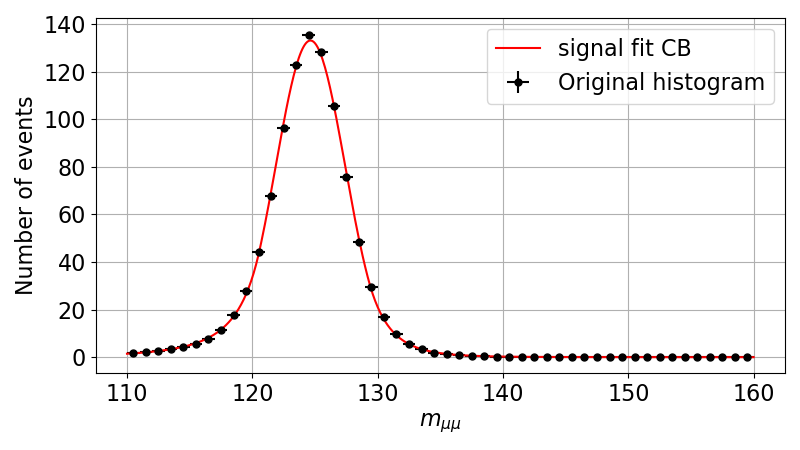
\includegraphics[width=\linewidth]{Pictures/CBfit.png}
\end{subfigure}
\caption*{Crystal Ball fit.}
\label{fig:CBfit}
\end{figure}

\section*{All together}
So we have played and got familiar with various methods of regression. Now we put it all together to find Higgs'. For this section, similar methods as in CERN are employed (using new methods would be too time consuming for this report)

First we fit the simulated background, this time by an ATLAS function, that is also commonly used in CERN (we find the best fit for the free parameter with curvefit). We can see that it fits very nicely:
\begin{figure}[H]
\centering
\begin{subfigure}{.7\textwidth}
\includegraphics[width=\linewidth]{Pictures/SimBkg_fit.pdf}
\end{subfigure}
\caption*{Simulated background ATLAS fit.}
\end{figure}

Next we do the same fit on the actual data except blind the data region $[120,130]$ (so Higgs' signal is not part of our fit). Result:
\begin{figure}[H]
\centering
\begin{subfigure}{.7\textwidth}
\includegraphics[width=\linewidth]{Pictures/DataBkg_fit.pdf}
\end{subfigure}
\caption*{Blinded data background ATLAS fit.}
\end{figure}

Next we extract the signal by simply subtracting the real data from the blinded background fit:
\begin{figure}[H]
\centering
\begin{subfigure}{.7\textwidth}
\includegraphics[width=\linewidth]{Pictures/Extracted_signal.pdf}
\end{subfigure}
\caption*{Data - Background fit}
\end{figure}

Next, we first fit the simulated signal to our CB function, again using curvefit:
\begin{figure}[H]
\centering
\begin{subfigure}{.7\textwidth}
\includegraphics[width=\linewidth]{Pictures/CB_fit.pdf}
\end{subfigure}
\caption*{Fitting CB to simulated signal}
\end{figure}

Finally, we fit the CB function also to our extracted signal:
\begin{figure}[H]
\centering
\begin{subfigure}{.7\textwidth}
\includegraphics[width=\linewidth]{Pictures/final_fit.pdf}
\end{subfigure}
\caption*{Fitting CB to signal}
\end{figure}

Removing the irrelevant background processes, we managed to find a signal that is a good fit for the theoretically motivated CB function at the mass of about 135. We have found the Higgs' boson.
\end{document}
